
%(BEGIN_QUESTION)
% Copyright 2011, Tony R. Kuphaldt, released under the Creative Commons Attribution License (v 1.0)
% This means you may do almost anything with this work of mine, so long as you give me proper credit

An engineer designs the following liquid level control system using a pair of split-ranged control valves.  His goal is to ensure the pump is never ``dead-headed'' (i.e. never pumping into a fully-shut control valve), but rather is always pumping liquid {\it somewhere}, whether it be away from the tank or recycling back to the tank:

$$\includegraphics[width=15.5cm]{i00892x01.eps}$$

Unfortunately, this system has a design flaw.  Recommend a suggestion that will fix the design flaw:

\underbar{file i00892}
%(END_QUESTION)





%(BEGIN_ANSWER)

{\bf The split-ranging is incorrect: it should be complementary, not exclusive.}  Actually, any answer that overlaps the valves' split-ranges is a good answer, and deserves full credit.

\vskip 10pt

\noindent
{\bf Explanation of problem:} the way it stands right now, there is still a possibility that the pump will be dead-headed: when the controller output is 50\%.  Also, the lower half of the controller's range is completely useless: the recycle valve will do absolutely nothing to control level no matter what it's position, so long as the outgoing valve is shut!

%(END_ANSWER)





%(BEGIN_NOTES)

{\bf This question is intended for exams only and not worksheets!}.

%(END_NOTES)


